\documentclass{ximera}  

%\usepackage{todonotes}
%\usepackage{mathtools} %% Required for wide table Curl and Greens
%\usepackage{cuted} %% Required for wide table Curl and Greens
\newcommand{\todo}{}

\usepackage{esint} % for \oiint
\ifxake%%https://math.meta.stackexchange.com/questions/9973/how-do-you-render-a-closed-surface-double-integral
\renewcommand{\oiint}{{\large\bigcirc}\kern-1.56em\iint}
\fi


\graphicspath{
  {./}
  {jpg}
  {ximeraTutorial/}
  {basicPhilosophy/}
  {functionsOfSeveralVariables/}
  {normalVectors/}
  {lagrangeMultipliers/}
  {vectorFields/}
  {greensTheorem/}
  {shapeOfThingsToCome/}
  {dotProducts/}
  {partialDerivativesAndTheGradientVector/}
  {../productAndQuotientRules/exercises/}
  {../motionAndPathsInSpace/exercises/}
  {../normalVectors/exercisesParametricPlots/}
  {../continuityOfFunctionsOfSeveralVariables/exercises/}
  {../partialDerivativesAndTheGradientVector/exercises/}
  {../directionalDerivativeAndChainRule/exercises/}
  {../commonCoordinates/exercisesCylindricalCoordinates/}
  {../commonCoordinates/exercisesSphericalCoordinates/}
  {../greensTheorem/exercisesCurlAndLineIntegrals/}
  {../greensTheorem/exercisesDivergenceAndLineIntegrals/}
  {../shapeOfThingsToCome/exercisesDivergenceTheorem/}
  {../greensTheorem/}
  {../shapeOfThingsToCome/}
  {../separableDifferentialEquations/exercises/}
  {vectorFields/}
}

\newcommand{\mooculus}{\textsf{\textbf{MOOC}\textnormal{\textsf{ULUS}}}}

\usepackage{tkz-euclide}\usepackage{tikz}
\usepackage{tikz-cd}
\usetikzlibrary{arrows}
\tikzset{>=stealth,commutative diagrams/.cd,
  arrow style=tikz,diagrams={>=stealth}} %% cool arrow head
\tikzset{shorten <>/.style={ shorten >=#1, shorten <=#1 } } %% allows shorter vectors

\usetikzlibrary{backgrounds} %% for boxes around graphs
\usetikzlibrary{shapes,positioning}  %% Clouds and stars
\usetikzlibrary{matrix} %% for matrix
\usepgfplotslibrary{polar} %% for polar plots
\usepgfplotslibrary{fillbetween} %% to shade area between curves in TikZ
\usetkzobj{all}
\usepackage[makeroom]{cancel} %% for strike outs
%\usepackage{mathtools} %% for pretty underbrace % Breaks Ximera
%\usepackage{multicol}
\usepackage{pgffor} %% required for integral for loops



%% http://tex.stackexchange.com/questions/66490/drawing-a-tikz-arc-specifying-the-center
%% Draws beach ball
\tikzset{pics/carc/.style args={#1:#2:#3}{code={\draw[pic actions] (#1:#3) arc(#1:#2:#3);}}}



\usepackage{array}
\setlength{\extrarowheight}{+.1cm}
\newdimen\digitwidth
\settowidth\digitwidth{9}
\def\divrule#1#2{
\noalign{\moveright#1\digitwidth
\vbox{\hrule width#2\digitwidth}}}





\newcommand{\RR}{\mathbb R}
\newcommand{\R}{\mathbb R}
\newcommand{\N}{\mathbb N}
\newcommand{\Z}{\mathbb Z}

\newcommand{\sagemath}{\textsf{SageMath}}


%\renewcommand{\d}{\,d\!}
\renewcommand{\d}{\mathop{}\!d}
\newcommand{\dd}[2][]{\frac{\d #1}{\d #2}}
\newcommand{\pp}[2][]{\frac{\partial #1}{\partial #2}}
\renewcommand{\l}{\ell}
\newcommand{\ddx}{\frac{d}{\d x}}

\newcommand{\zeroOverZero}{\ensuremath{\boldsymbol{\tfrac{0}{0}}}}
\newcommand{\inftyOverInfty}{\ensuremath{\boldsymbol{\tfrac{\infty}{\infty}}}}
\newcommand{\zeroOverInfty}{\ensuremath{\boldsymbol{\tfrac{0}{\infty}}}}
\newcommand{\zeroTimesInfty}{\ensuremath{\small\boldsymbol{0\cdot \infty}}}
\newcommand{\inftyMinusInfty}{\ensuremath{\small\boldsymbol{\infty - \infty}}}
\newcommand{\oneToInfty}{\ensuremath{\boldsymbol{1^\infty}}}
\newcommand{\zeroToZero}{\ensuremath{\boldsymbol{0^0}}}
\newcommand{\inftyToZero}{\ensuremath{\boldsymbol{\infty^0}}}



\newcommand{\numOverZero}{\ensuremath{\boldsymbol{\tfrac{\#}{0}}}}
\newcommand{\dfn}{\textbf}
%\newcommand{\unit}{\,\mathrm}
\newcommand{\unit}{\mathop{}\!\mathrm}
\newcommand{\eval}[1]{\bigg[ #1 \bigg]}
\newcommand{\seq}[1]{\left( #1 \right)}
\renewcommand{\epsilon}{\varepsilon}
\renewcommand{\phi}{\varphi}


\renewcommand{\iff}{\Leftrightarrow}

\DeclareMathOperator{\arccot}{arccot}
\DeclareMathOperator{\arcsec}{arcsec}
\DeclareMathOperator{\arccsc}{arccsc}
\DeclareMathOperator{\si}{Si}
\DeclareMathOperator{\scal}{scal}
\DeclareMathOperator{\sign}{sign}


%% \newcommand{\tightoverset}[2]{% for arrow vec
%%   \mathop{#2}\limits^{\vbox to -.5ex{\kern-0.75ex\hbox{$#1$}\vss}}}
\newcommand{\arrowvec}[1]{{\overset{\rightharpoonup}{#1}}}
%\renewcommand{\vec}[1]{\arrowvec{\mathbf{#1}}}
\renewcommand{\vec}[1]{{\overset{\boldsymbol{\rightharpoonup}}{\mathbf{#1}}}\hspace{0in}}

\newcommand{\point}[1]{\left(#1\right)} %this allows \vector{ to be changed to \vector{ with a quick find and replace
\newcommand{\pt}[1]{\mathbf{#1}} %this allows \vec{ to be changed to \vec{ with a quick find and replace
\newcommand{\Lim}[2]{\lim_{\point{#1} \to \point{#2}}} %Bart, I changed this to point since I want to use it.  It runs through both of the exercise and exerciseE files in limits section, which is why it was in each document to start with.

\DeclareMathOperator{\proj}{\mathbf{proj}}
\newcommand{\veci}{{\boldsymbol{\hat{\imath}}}}
\newcommand{\vecj}{{\boldsymbol{\hat{\jmath}}}}
\newcommand{\veck}{{\boldsymbol{\hat{k}}}}
\newcommand{\vecl}{\vec{\boldsymbol{\l}}}
\newcommand{\uvec}[1]{\mathbf{\hat{#1}}}
\newcommand{\utan}{\mathbf{\hat{t}}}
\newcommand{\unormal}{\mathbf{\hat{n}}}
\newcommand{\ubinormal}{\mathbf{\hat{b}}}

\newcommand{\dotp}{\bullet}
\newcommand{\cross}{\boldsymbol\times}
\newcommand{\grad}{\boldsymbol\nabla}
\newcommand{\divergence}{\grad\dotp}
\newcommand{\curl}{\grad\cross}
%\DeclareMathOperator{\divergence}{divergence}
%\DeclareMathOperator{\curl}[1]{\grad\cross #1}
\newcommand{\lto}{\mathop{\longrightarrow\,}\limits}

\renewcommand{\bar}{\overline}

\colorlet{textColor}{black}
\colorlet{background}{white}
\colorlet{penColor}{blue!50!black} % Color of a curve in a plot
\colorlet{penColor2}{red!50!black}% Color of a curve in a plot
\colorlet{penColor3}{red!50!blue} % Color of a curve in a plot
\colorlet{penColor4}{green!50!black} % Color of a curve in a plot
\colorlet{penColor5}{orange!80!black} % Color of a curve in a plot
\colorlet{penColor6}{yellow!70!black} % Color of a curve in a plot
\colorlet{fill1}{penColor!20} % Color of fill in a plot
\colorlet{fill2}{penColor2!20} % Color of fill in a plot
\colorlet{fillp}{fill1} % Color of positive area
\colorlet{filln}{penColor2!20} % Color of negative area
\colorlet{fill3}{penColor3!20} % Fill
\colorlet{fill4}{penColor4!20} % Fill
\colorlet{fill5}{penColor5!20} % Fill
\colorlet{gridColor}{gray!50} % Color of grid in a plot

\newcommand{\surfaceColor}{violet}
\newcommand{\surfaceColorTwo}{redyellow}
\newcommand{\sliceColor}{greenyellow}




\pgfmathdeclarefunction{gauss}{2}{% gives gaussian
  \pgfmathparse{1/(#2*sqrt(2*pi))*exp(-((x-#1)^2)/(2*#2^2))}%
}


%%%%%%%%%%%%%
%% Vectors
%%%%%%%%%%%%%

%% Simple horiz vectors
\renewcommand{\vector}[1]{\left\langle #1\right\rangle}


%% %% Complex Horiz Vectors with angle brackets
%% \makeatletter
%% \renewcommand{\vector}[2][ , ]{\left\langle%
%%   \def\nextitem{\def\nextitem{#1}}%
%%   \@for \el:=#2\do{\nextitem\el}\right\rangle%
%% }
%% \makeatother

%% %% Vertical Vectors
%% \def\vector#1{\begin{bmatrix}\vecListA#1,,\end{bmatrix}}
%% \def\vecListA#1,{\if,#1,\else #1\cr \expandafter \vecListA \fi}

%%%%%%%%%%%%%
%% End of vectors
%%%%%%%%%%%%%

%\newcommand{\fullwidth}{}
%\newcommand{\normalwidth}{}



%% makes a snazzy t-chart for evaluating functions
%\newenvironment{tchart}{\rowcolors{2}{}{background!90!textColor}\array}{\endarray}

%%This is to help with formatting on future title pages.
\newenvironment{sectionOutcomes}{}{}



%% Flowchart stuff
%\tikzstyle{startstop} = [rectangle, rounded corners, minimum width=3cm, minimum height=1cm,text centered, draw=black]
%\tikzstyle{question} = [rectangle, minimum width=3cm, minimum height=1cm, text centered, draw=black]
%\tikzstyle{decision} = [trapezium, trapezium left angle=70, trapezium right angle=110, minimum width=3cm, minimum height=1cm, text centered, draw=black]
%\tikzstyle{question} = [rectangle, rounded corners, minimum width=3cm, minimum height=1cm,text centered, draw=black]
%\tikzstyle{process} = [rectangle, minimum width=3cm, minimum height=1cm, text centered, draw=black]
%\tikzstyle{decision} = [trapezium, trapezium left angle=70, trapezium right angle=110, minimum width=3cm, minimum height=1cm, text centered, draw=black]




 
\title{Review of Complex Numbers} 
\author{Milica Markovic} 
\begin{document}  
\begin{abstract}  
Invest time in studying complex numbers, because phasors are represented with complex numbers!
\end{abstract}  
\maketitle    
  
  \begin{definition}
 A complex number  $z$ can be represented in Cartesian coordinate system as shown in Equation \ref{cartesian}, and  Polar coordinate system as shown in Equation \ref{polar}. 




\begin{eqnarray}
z= x + j y \label{cartesian} \\ 
z=|z| e^{j \Theta} \label{polar}
\end{eqnarray}

\end{definition}

In Equation \ref{cartesian}, a complex number z is represented in rectangular coordinate system, where $x$ is the real part, $y$ is the imaginary part, and $j=\sqrt{-1}$. 

In Equation \ref{polar}, a complex number z is represented in polar coordinate system, where  $|z|$ is the magnitude and $\Theta$ is the angle (aka phase) of the complex number.

Geometric interpretation of these two equations is given in Figure \ref{wind}. The magnitude is the length of the hypothenuse of the triangle shown, and the angle is the angle that the hypothenuse makes with x-axis. 
\begin{figure}[htbp]
\begin{center}
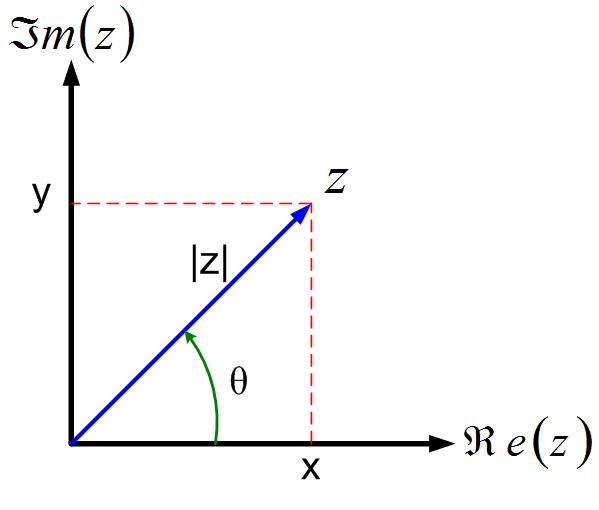
\includegraphics[scale=0.3]{../jpg/Complex_Numbersz12.jpg}
%\strut\psfig{figure=complexnumberz.ps,width=3cm} \\
\end{center}
\caption{Visual representation of a complex number z in rectangular $z=x+jy$ and polar coordinates $z=|z|e^{j \theta}$.}
\label{wind}
\end{figure}




You may be wondering why are we representing the phase of a complex number in polar coordinate system as  $e^{j \Theta}$, because in the circuits class you used $\angle \theta$. Great question. That brings us to Eurler's formula.

  
 \subsection{Euler's formula} 
  
  

 Euler's formula relates the Cartesian and Polar coordinates for complex numbers.

\begin{eqnarray}
e^{j \Theta} = cos \Theta + j sin \Theta
\end{eqnarray}

Geometric interpretation of the Euler's formula is shown below. $z=r ( \cos{\theta} + j \sin{\theta})$, where $r \cos{\theta}=x$ and $r \sin{\theta}=y$. Euler's formula shows that number z given in Cartesian coordinates as $x+jy$ can be represented in Polar Coordinates as   $e^{j \Theta}$. You have likely seen this proof in your Calculus class.  {\bf TIP: Your calculator may not know what $e^{j\theta}$ is. Check how to convert between polar and cartesian coordinates on your calculatorbefore the test.}


  \begin{image}
\begin{tikzpicture}
	\begin{axis}[
            xmin=-1.1,xmax=1.1,ymin=-1.1,ymax=1.1,
            axis lines=center,
            width=4in,
            xtick={-1,1},
            ytick={-1,1},
            clip=false,
            unit vector ratio*=1 1 1,
            xlabel=$x$, ylabel=$y$,
            every axis y label/.style={at=(current axis.above origin),anchor=south},
            every axis x label/.style={at=(current axis.right of origin),anchor=west},
          ]        
          \addplot [dashed, smooth, domain=(0:360)] ({cos(x)},{sin(x)}); %% unit circle

          \addplot [textColor] plot coordinates {(0,0) (.766,.643)}; %% 40 degrees

          \addplot [ultra thick,penColor] plot coordinates {(.766,0) (.766,.643)}; %% 40 degrees
          \addplot [ultra thick,penColor2] plot coordinates {(0,0) (.766,0)}; %% 40 degrees
          
          %\addplot [ultra thick,penColor3] plot coordinates {(1,0) (1,.839)}; %% 40 degrees          

          \addplot [textColor,smooth, domain=(0:40)] ({.15*cos(x)},{.15*sin(x)});
          %\addplot [very thick,penColor] plot coordinates {(0,0) (.766,.643)}; %% sector
          %\addplot [very thick,penColor] plot coordinates {(0,0) (1,0)}; %% sector
          %\addplot [very thick, penColor, smooth, domain=(0:40)] ({cos(x)},{sin(x)}); %% sector
          \node at (axis cs:.15,.07) [anchor=west] {$\theta$};
          \node[penColor, rotate=-90] at (axis cs:.84,.322) {$\sin(\theta)$};
          \node[penColor2] at (axis cs:.383,0) [anchor=north] {$\cos(\theta)$};
          %\node[penColor3, rotate=-90] at (axis cs:1.06,.322) {$\tan(\theta)$};
        \end{axis}
\end{tikzpicture}
\end{image}
  
  
 
  
  To find magnitude and angle when you know real and imaginary part of a complex number, 

\begin{eqnarray}
|z|=\sqrt{x^2+y^2} \\
\Theta = arctg \frac{y}{x}
\end{eqnarray}

\section{Operations with complex numbers}

 Complex Conjugate is often seen when finding the conditions for maximum power transfer.

\begin{eqnarray}
z^* = (x+ j y)^* = x- j y = |z| e^{-j \Theta}
\end{eqnarray}


 Complex number addition and subtraction is often seen went to complex impedances are placed in series and the equivalent  complex impedance has to be found. the easiest way to add two complex numbers is to find Cartesian representation of both and then add the real parts separately and the imaginary part separately.

\begin{eqnarray}
z_1=x_1 + j y_1 \\
z_2=x_2 + j y_2 \\
z_1+z_2 = x_1 + x_2 + j ( y_1 + y_2)
\end{eqnarray}

Multiplication and Division are often seen the in calculation of the transfer function of a circuit. The easiest way to divide two complex numbers is to find the polar representation of both and then divide the amplitudes  and subtract the phases.

\begin{eqnarray}
z_1=|z_1| e^{j \Theta_1} \\
z_2=|z_2| e^{j \Theta_2} \\
\frac{z_1}{ z_2} = \frac{|z_1|}{|z_2|} e^{j \Theta_1 -\Theta_2}
\end{eqnarray}
  


 

\begin{example}
Find the magnitude and phase of a complex numbers $z_1=j$ and $z_2=1$.


\begin{explanation}

Complex number $z_1=j$ is on the y-axis where y=1. By inspection, the magnitude 
     of $z_1$ is $|z|=1$, and the angle is $\theta=90^o$.



  \begin{image}
\begin{tikzpicture}
	\begin{axis}[
            xmin=-1.1,xmax=1.1,ymin=-1.1,ymax=1.1,
            axis lines=center,
            width=4in,
            xtick={-1,1},
            ytick={-1,1},
            clip=false,
            unit vector ratio*=1 1 1,
            xlabel=$x$, ylabel=$y$,
            every axis y label/.style={at=(current axis.above origin),anchor=south},
            every axis x label/.style={at=(current axis.right of origin),anchor=west},
          ]        
        %  \addplot [dashed, smooth, domain=(0:360)] ({cos(x)},{sin(x)}); %% unit circle

          \addplot [textColor] plot coordinates {(0,0) (0,1)}; %% 90 degrees

          %vertical red up line from 0,0 to 0,1
          \addplot [ultra thick,penColor2] plot coordinates {(0,0) (0,1)}; %% 90 degrees
          
         % draw small circle to designate that theta is 90 degrees        

          \addplot [textColor,smooth, domain=(0:90)] ({.15*cos(x)},{.15*sin(x)});
          % write theta next to the small circle
         
          \node at (axis cs:.11,.11) [anchor=west] {$\theta$};
          %write j next to the y=1
         
          \node at (axis cs:0.35,1) [anchor=east] {$z=j$};
          
        \end{axis}
\end{tikzpicture}
\end{image}
  

Complex plane is sketched below.
Complex number $z_1=1$ is on the x-axis where x=1. By inspection, the magnitude 
     of $z_1$ is $|z|=1$, and the angle is $\theta=0^o$.


  \begin{image}
\begin{tikzpicture}
	\begin{axis}[
            xmin=-1.1,xmax=1.1,ymin=-1.1,ymax=1.1,
            axis lines=center,
            width=4in,
            xtick={-1,1},
            ytick={-1,1},
            clip=false,
            unit vector ratio*=1 1 1,
            xlabel=$x$, ylabel=$y$,
            every axis y label/.style={at=(current axis.above origin),anchor=south},
            every axis x label/.style={at=(current axis.right of origin),anchor=west},
          ]        
        %  \addplot [dashed, smooth, domain=(0:360)] ({cos(x)},{sin(x)}); %% unit circle

          \addplot [textColor] plot coordinates {(0,0) (0,1)}; %% 90 degrees

          %horizontal red up line from 0,0 to 0,1
          \addplot [ultra thick,penColor2] plot coordinates {(0,0) (1,0)}; %% 0 degrees
          
         % draw small circle to designate that theta is 90 degrees        

      %    \addplot [textColor,smooth, domain=(0:90)] ({.15*cos(x)},{.15*sin(x)});
          % write theta next to the small circle
         
    %      \node at (axis cs:.11,.11) [anchor=west] {$\theta$};
          %write j next to the y=1
         
          \node at (axis cs:1,0) [anchor=south] {$z=1$};
          
        \end{axis}
\end{tikzpicture}
\end{image}


\end{explanation}
\end{example}


\begin{question}
Calculate magnitude and phase of 
complex number $z=-j$ 
\begin{multipleChoice}  
\choice{$|z|= 1, \theta={180}$}
\choice[correct]{$|z|= 1, \theta={-90}$}   
\choice{$|z|= -1, \theta={180}$}
\choice{$|z|= -1,  \theta={-90}$}
\end{multipleChoice}
\end{question}
  
  
  
  
  
  
  
  
  
  
  
  
  
  
  
  
  
  
  
  
  
  
  
  Write magnitude and phase of complex number $z=-1$
\begin{question}  
         $ -1 =  \answer{e^{j180}}$  
    \end{question} 
    
    
    
    
    
    
    
    
    
    
    
    
    
    
    
    
    
    
    
\end{document} 
